\subsection{Quantization Error}
\label{subsec:quantization_error}

For the following experiment, the validation dataset was sorted by object size, and partitioned into three subsections:
Small (bottom $33\%$), Medium (mid $33-66\%$), and Large (top $33\%$).

\subsubsection*{Results}

\begin{figure}[h]
    \centering
    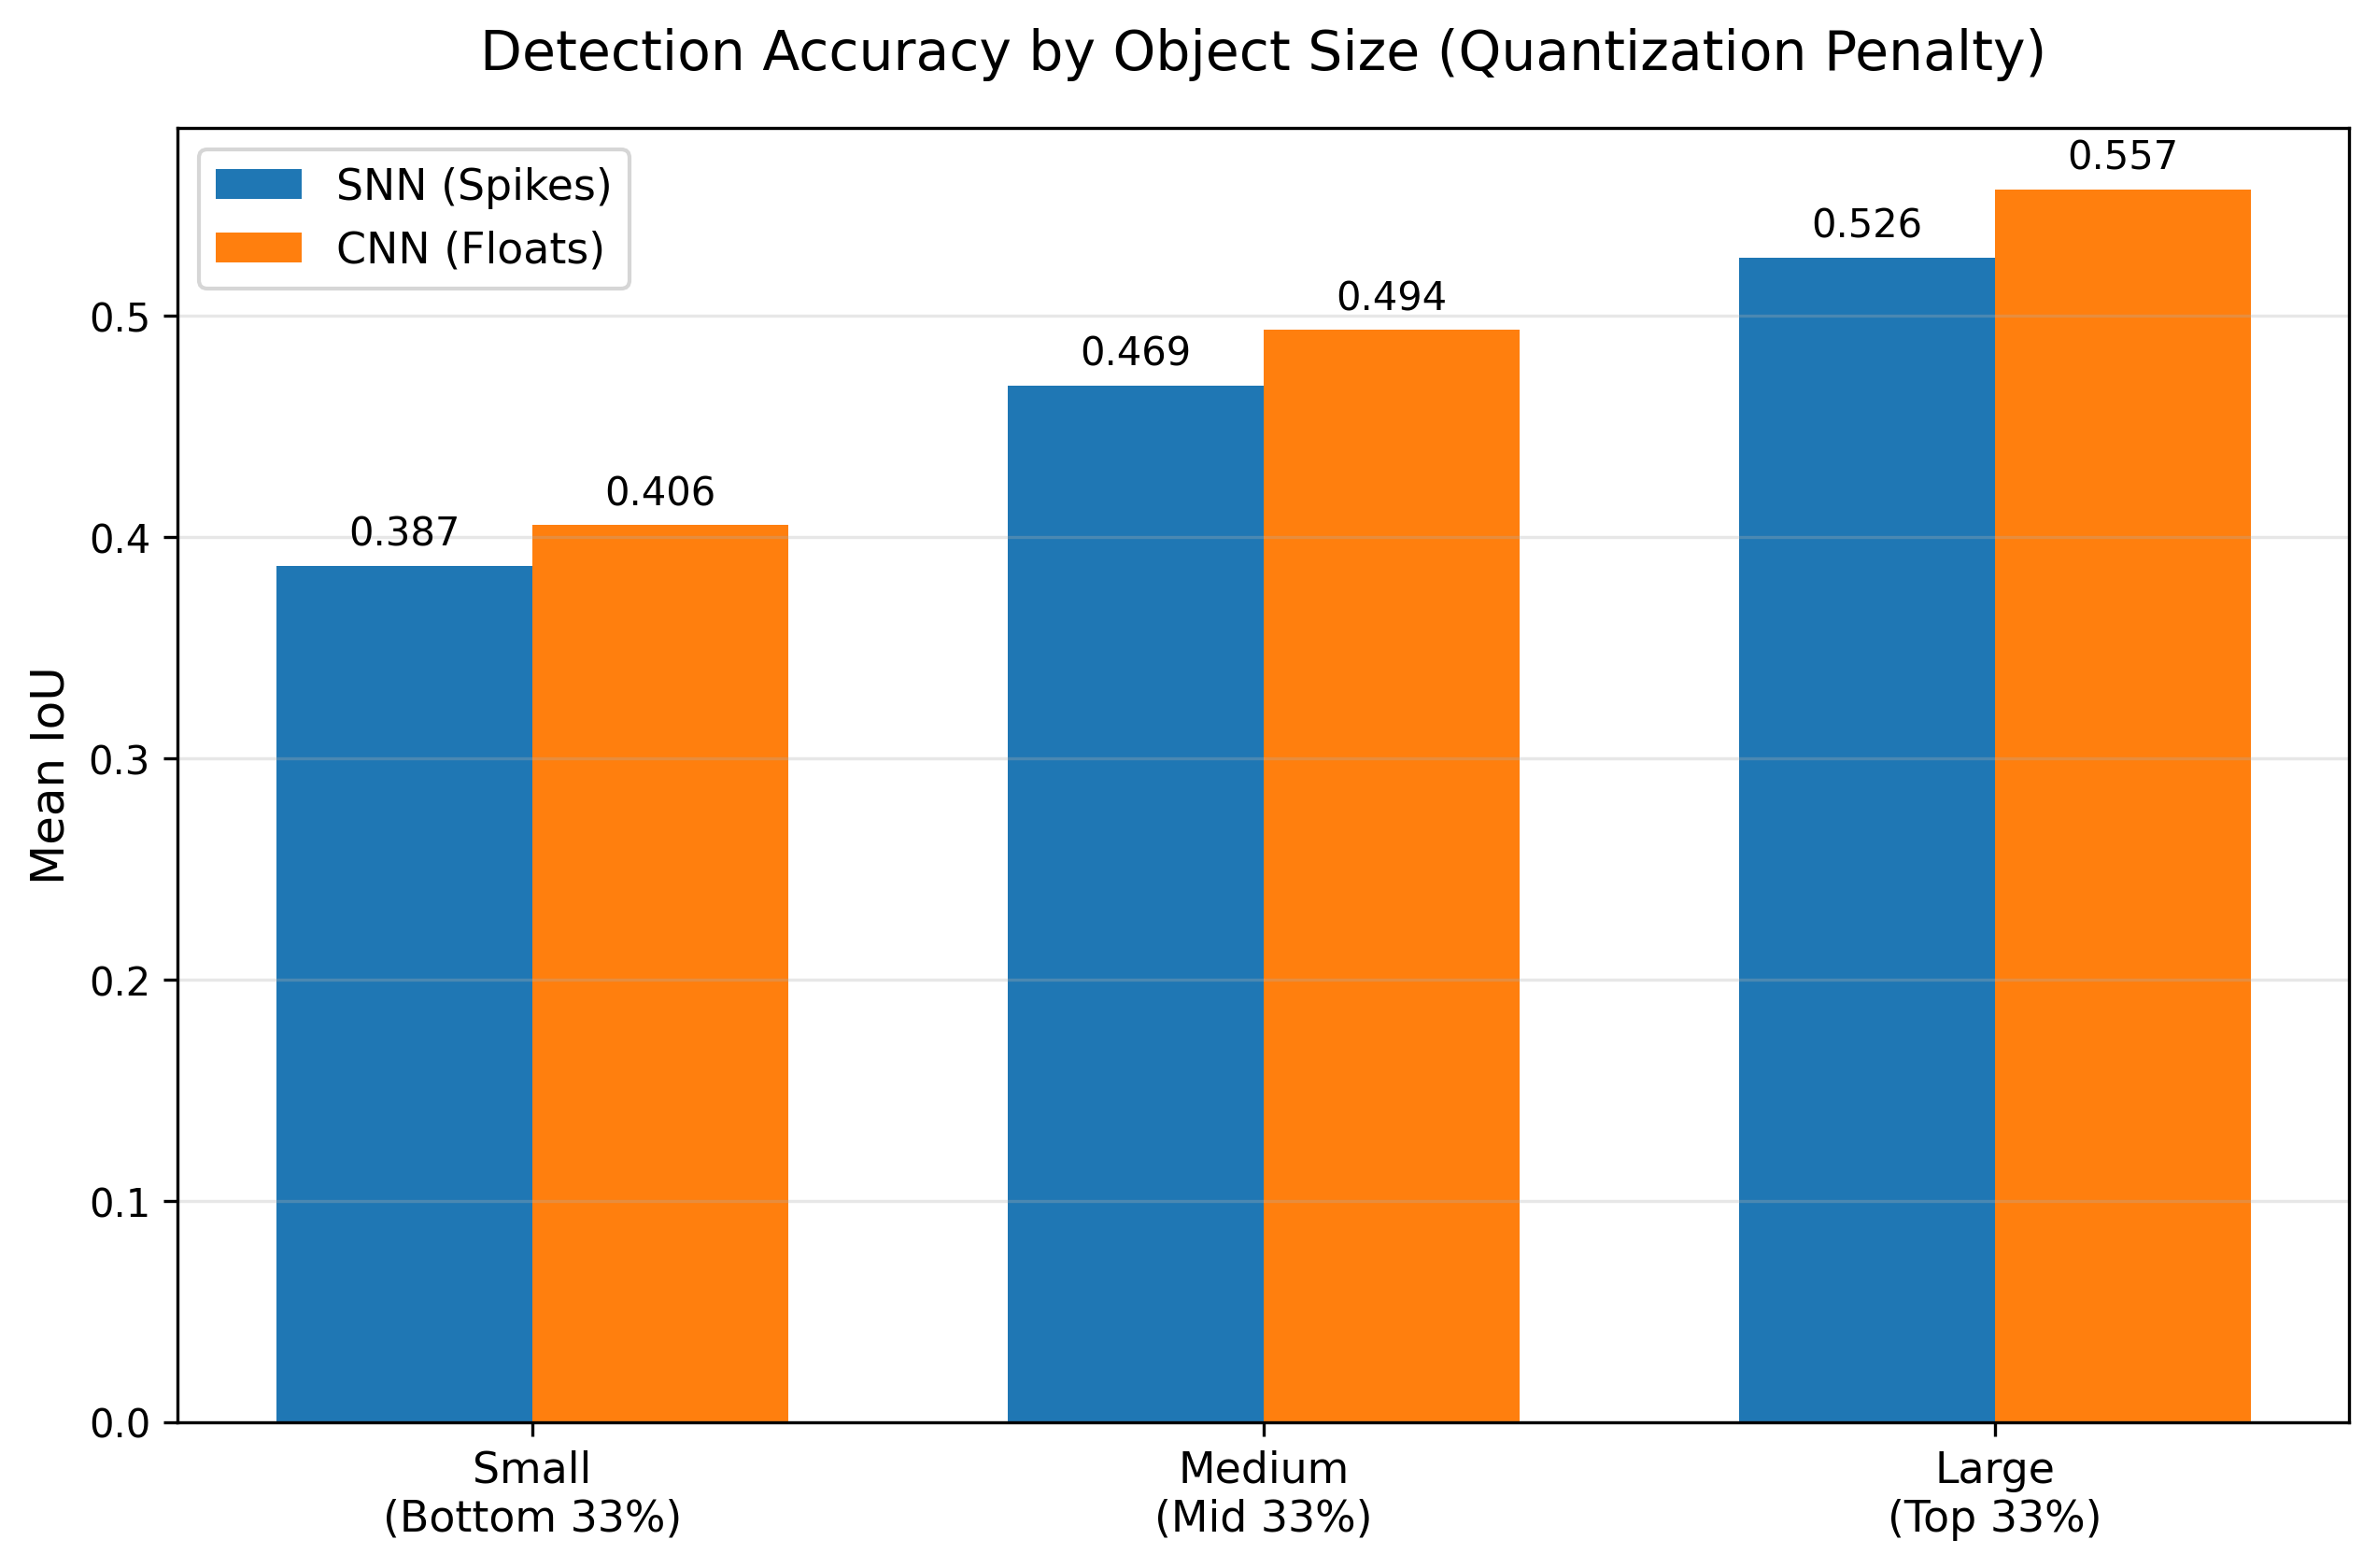
\includegraphics[width=\textwidth]{chapter_3/dnx_results/exp2_accuracy_vs_size.png}
    \caption{Quantization Error Analysis (Accuracy vs. Object Size) of \gls{snn} (Blue) and \gls{cnn} (Orange).}
    \label{fig:quantization_error}
\end{figure}

Figure \ref{fig:quantization_error} illustrates the performance of the \gls{snn} and \gls{cnn} models on the three object size categories;
it shows the Mean \gls{iou} of both models across all samples in each subset.

\begin{table}[h]
    \centering
    \begin{tabular}{|l|c|c|c|}
        \hline
        \textbf{Object Size} & \textbf{SNN \gls{miou} Drop} & \textbf{SNN \gls{miou} Drop (\%)} \\
        \hline
        Small & 0.019 & 4.7 \\
        Medium & 0.025 & 5.1 \\
        Large & 0.031 & 5.6 \\
        \hline
    \end{tabular}
    \caption{Quantization Error Analysis showing drop in \gls{snn} performance against \gls{cnn}.}
    \label{tab:quantization_error}
\end{table}

\subsubsection*{Critical Analysis}

Earlier in Section \ref{subsubsec:quant_hyp}, we hypothesized the idea of a scale-dependent accuracy gap,
where the 1-bit quantization error would disproportionately penalise the \gls{snn} on small objects
(because a 1-pixel rounding error is massive for a tiny car) and achieve parity on large objects.

However, the empirical results in Table \ref{tab:quantization_error} present an inverse trend, invalidating the expected scale-dependent penalty.
The \gls{snn} proved most competitive on the smallest validation targets, with a performance drop of only $4.7\%$.
This resilience suggests that the multi-box architectural refinements detailed in Section \ref{sec:architectural_evolution}
successfully preserved local spatial context, effectively insulating small-scale features from the discrete quantization error.

Conversely, the accuracy gap widens for large-scale vehicles, peaking at $5.6\%$.
This divergence suggests that the quantization error instead acts as a global geometric bottleneck rather than a scale-dependent failure:
on large objects where high-definition event volumes provide sufficient data for precise edge-refinement,
the continuous floating-point activations of the \gls{cnn} allow for infinite coordinate adjustments.
In contrast, the \gls{snn} is physically constrained by its 11 representable states ($T=10$), 
resulting in a persistent geometric drag that prevents the same level of fine-grained bounding box alignment achievable by the baseline.
Had the temporal simulation window been reduced further (e.g. $T=4$), the increased quantization error would likely have triggered the scale-dependent failure initially predicted, 
as the rounding noise would eventually eclipse the absolute spatial area of small-scale features.

In summary, We can conclude that while the \gls{snn} is a robust macro-level detector, in its current configuration the discrete temporal resolution
imposes a fundamental precision ceiling across all global scales, instead of a scale-dependent one.